% Created 2020-08-24 lun. 18:19
% Intended LaTeX compiler: pdflatex
\documentclass[t, minted]{clean-beamer}
\usepackage[utf8]{inputenc}
\usepackage[T1]{fontenc}
\usepackage{graphicx}
\usepackage{grffile}
\usepackage{longtable}
\usepackage{wrapfig}
\usepackage{rotating}
\usepackage[normalem]{ulem}
\usepackage{amsmath}
\usepackage{textcomp}
\usepackage{amssymb}
\usepackage{capt-of}
\usepackage{hyperref}
\usepackage[most]{tcolorbox}
\usepackage{bm}
\usepackage{booktabs}
\usepackage{tabularx}
\usepackage{array}
\usepackage{siunitx}
\usepackage{tikz}
\usetikzlibrary{decorations.text}
\author[shortname]{Thomas Dehaeze \inst{1,3} \and Christophe Collette \inst{1,2}}
\institute[shortinst]{\inst{1} Precision Mechatronics Laboratory, University of Liege, Belgium \and %
\inst{2} BEAMS Department, Free University of Brussels, Belgium \and %
\inst{3} European Synchrotron Radiation Facility, Grenoble, France}
\titlegraphic{\includegraphics[height=1.5cm]{figs/logo_pml.png} \hspace{5em} %
\includegraphics[height=1.5cm]{figs/logo_esrf.png} \hspace{5em} %
\includegraphics[height=1.5cm]{figs/logo_isma.png}}
\beamertemplatenavigationsymbolsempty
\addtobeamertemplate{navigation symbols}{}{%
\usebeamerfont{footline}%
\usebeamercolor[fg]{footline}%
\hspace{1em}%
\insertframenumber/\inserttotalframenumber
}
\setbeamertemplate{itemize items}[circle]
\usefonttheme[onlymath]{serif}
\AtBeginSection[]{
\begin{frame}<beamer>{Outline}
\tableofcontents[currentsection, hideothersubsections, sectionstyle=show/shaded]
\end{frame}
}
\usetheme{default}
\date{}
\title{Active Damping of Rotating Platforms using Integral Force Feedback}
\subtitle{ISMA-USD 2020, September 7-9, 2020}
\hypersetup{
 pdfauthor={},
 pdftitle={Active Damping of Rotating Platforms using Integral Force Feedback},
 pdfkeywords={},
 pdfsubject={},
 pdfcreator={Emacs 27.1.50 (Org mode 9.4)}, 
 pdflang={English}}
\begin{document}

\maketitle
\begin{frame}{Outline}
\tableofcontents
\end{frame}


\section{Dynamics of Rotating Platforms}
\label{sec:orge3e010f}
\begin{frame}[label={sec:orgac66c89}]{Model of a Rotating Positioning Platform}
\begin{figure}[htbp]
\centering
\includegraphics[width=0.7\linewidth]{figs/system.pdf}
\caption{Schematic of the studied System}
\end{figure}
\end{frame}

\begin{frame}[label={sec:org614e76f}]{Equations of Motion - Lagrangian Formalism}
Lagrangian equations:
\begin{equation*}
  \frac{d}{dt} \left( \frac{\partial L}{\partial \dot{q}_i} \right) + \frac{\partial D}{\partial \dot{q}_i} - \frac{\partial L}{\partial q_i} = Q_i
\end{equation*}

\vspace{1em}

Equations of motion:
\begin{align*}
  m \ddot{d}_u + c \dot{d}_u + ( k - m \Omega^2 ) d_u &= F_u + 2 m \Omega \dot{d}_v \\
  m \ddot{d}_v + c \dot{d}_v + ( k \underbrace{-\,m \Omega^2}_{\text{Centrif.}} ) d_v &= F_v \underbrace{-\,2 m \Omega \dot{d}_u}_{\text{Coriolis}}
\end{align*}

\vspace{1em}

\begin{cbox}[]{blue}{}
\begin{center}
Centrifugal forces \(\Longleftrightarrow\) Negative Stiffness

Coriolis Forces \(\Longleftrightarrow\) Coupling
\end{center}
\end{cbox}
\end{frame}

\begin{frame}[label={sec:org0a25ba1}]{Transfer Function Matrix the Laplace domain}
\vspace{2em}

\begin{figure}[htbp]
\begin{subfigure}[c]{0.49\linewidth}
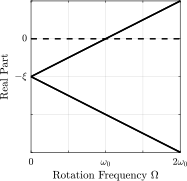
\includegraphics[width=\linewidth]{figs/campbell_diagram_real.pdf}
\caption{\label{fig:campbell_diagram_real} Real Part}
\end{subfigure}
\hfill
\begin{subfigure}[c]{0.49\linewidth}
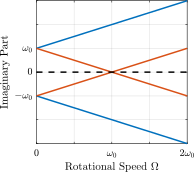
\includegraphics[width=\linewidth]{figs/campbell_diagram_imag.pdf}
\caption{\label{fig:campbell_diagram_imag} Imaginary Part}
\end{subfigure}
\hfill
\caption{Campbell Diagram : Evolution of the complex and real parts of the system's poles as a function of the rotational speed \(\Omega\)}
\centering
\end{figure}
\end{frame}

\section{Decentralized Integral Force Feedback}
\label{sec:org8107aa6}
\begin{frame}[label={sec:org818bd83}]{Force Sensors and Decentralized IFF Control Architecture}
\begin{figure}[htbp]
\centering
\includegraphics[width=0.7\linewidth]{figs/system_iff.pdf}
\caption{System with added Force Sensor in series with the actuators, \(K_F(s) = g \cdot \frac{1}{s}\)}
\end{figure}
\end{frame}

\begin{frame}[label={sec:org159eb7e}]{IFF Plant Dynamics}
\begin{figure}[htbp]
\centering
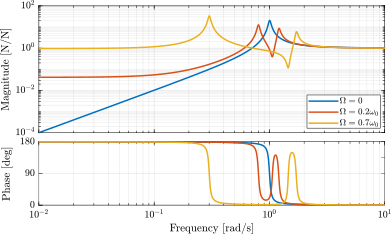
\includegraphics[width=\linewidth]{figs/plant_iff_compare_rotating_speed.pdf}
\caption{Bode plot of the dynamics from force actuator to force sensor for several rotational speeds \(\Omega\)}
\end{figure}
\end{frame}

\begin{frame}[label={sec:orge6035da}]{Decentralized IFF with Pure Integrators}
\begin{figure}[htbp]
\centering
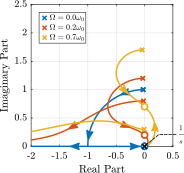
\includegraphics[width=0.7\linewidth]{figs/root_locus_pure_iff.pdf}
\caption{Root Locus for Decentralized IFF for several rotating speeds \(\Omega\)}
\end{figure}

\vspace{-1em}

\begin{cbox}[]{blue}{}
\centering For \(\Omega > 0\), the closed loop system is unstable
\end{cbox}
\end{frame}

\section{Integral Force Feedback with High Pass Filter}
\label{sec:org789619d}
\begin{frame}[label={sec:org2020343}]{Modification of the Control Law}
\begin{equation*}
  K_{F}(s) = g \cdot \frac{1}{s} \cdot \underbrace{\frac{s/\omega_i}{1 + s/\omega_i}}_{\text{HPF}} = g \cdot \frac{1}{s + \omega_i}
\end{equation*}

\vspace{1em}

\begin{minipage}[b]{0.45\linewidth}
\begin{center}
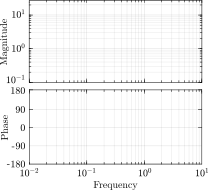
\includegraphics[width=\linewidth]{figs/loop_gain_modified_iff.pdf}
\captionof{figure}{Loop Gain}
\end{center}
\end{minipage}
\hfill
\begin{minipage}[b]{0.5\linewidth}
\begin{center}
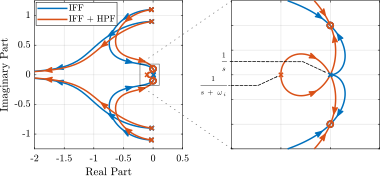
\includegraphics[width=\linewidth]{figs/root_locus_modified_iff.pdf}
\captionof{figure}{Root Locus}
\end{center}
\end{minipage}
\end{frame}


\begin{frame}[label={sec:org38b9bd2}]{Effect of \(\omega_i\) on the attainable damping}
\begin{figure}[htbp]
\centering
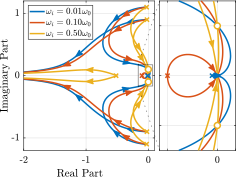
\includegraphics[width=\linewidth]{figs/root_locus_wi_modified_iff.pdf}
\caption{Root Locus for several HPF cut-off frequencies \(\omega_i\), \(\Omega = 0.1 \omega_0\)}
\end{figure}

\vspace{-2em}

\begin{columns}
\begin{column}{0.3\columnwidth}
\begin{equation*}
  g_{\text{max}} = \omega_i \left( \frac{{\omega_0}^2}{\Omega^2} - 1 \right)
\end{equation*}
\end{column}

\begin{column}{0.7\columnwidth}
\begin{cbox}[]{blue}{}
small \(\omega_i\) \(\Longrightarrow\) increase maximum damping

small \(\omega_i\) \(\Longrightarrow\) reduces maximum gain \(g_\text{max}\)
\end{cbox}
\end{column}
\end{columns}
\end{frame}

\begin{frame}[label={sec:orga2c2166}]{Optimal Control Parameters}
\vspace{1em}

\begin{figure}[htbp]
\centering
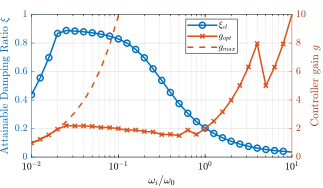
\includegraphics[width=\linewidth]{figs/mod_iff_damping_wi.pdf}
\caption{Attainable damping ratio \(\xi_\text{cl}\) as a function of the ratio \(\omega_i/\omega_0\). Corresponding control gain \(g_\text{opt}\) and \(g_\text{max}\) are also shown}
\end{figure}
\end{frame}

\section{Integral Force Feedback with Parallel Springs}
\label{sec:org7a61560}
\begin{frame}[label={sec:orga6be4f6}]{Stiffness in Parallel with the Force Sensor}
\begin{figure}[htbp]
\centering
\includegraphics[width=0.65\linewidth]{figs/system_parallel_springs.pdf}
\caption{System with additional springs in parallel with the actuators and force sensors}
\end{figure}
\end{frame}

\begin{frame}[label={sec:org497c282}]{Effect of the Parallel Stiffness on the Plant Dynamics}
\begin{minipage}[b]{0.42\linewidth}
\begin{figure}[htbp]
\centering
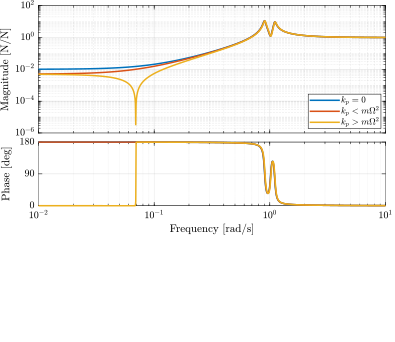
\includegraphics[width=\linewidth]{figs/plant_iff_kp.pdf}
\caption{Bode Plot of \(f_u/F_u\)}
\end{figure}
\end{minipage}
\hfill
\begin{minipage}[b]{0.55\linewidth}
\begin{figure}[htbp]
\centering
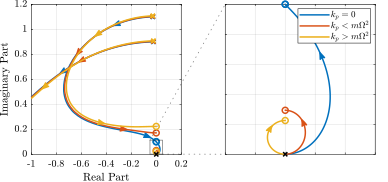
\includegraphics[width=\linewidth]{figs/root_locus_iff_kp.pdf}
\caption{Root Locus for IFF}
\end{figure}
\end{minipage}

\vspace{1em}

\begin{cbox}[]{blue}{}
If \(k_p > m \Omega^2\), the poles of the closed-loop system stay in the (stable) right half-plane, and hence the \textbf{unconditional stability of IFF is recovered}.
\end{cbox}
\end{frame}

\begin{frame}[label={sec:orgd7eccc9}]{Optimal Parallel Stiffness}
\begin{figure}[htbp]
\centering
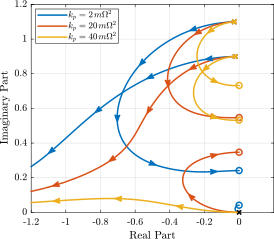
\includegraphics[width=0.60\linewidth]{figs/root_locus_iff_kps.pdf}
\caption{Root Locus for three parallel stiffnesses \(k_p\)}
\end{figure}

\begin{cbox}[]{blue}{}
\centering
Large parallel stiffness \(k_p\) reduces the attainable damping.
\end{cbox}
\end{frame}

\section{Comparison and Discussion}
\label{sec:org79d4359}
\begin{frame}[label={sec:org7dda174}]{Comparison of the Attainable Damping}
\begin{figure}[htbp]
\centering
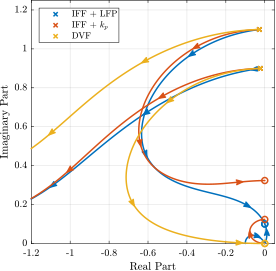
\includegraphics[width=0.7\linewidth]{figs/comp_root_locus.pdf}
\caption{Root Locus for the two proposed modifications of decentralized IFF, \(\Omega = 0.1 \omega_0\)}
\end{figure}
\end{frame}

\begin{frame}[label={sec:org9effb95}]{Comparison Transmissibility and Compliance}
\begin{figure}[htbp]
\begin{subfigure}[c]{0.49\linewidth}
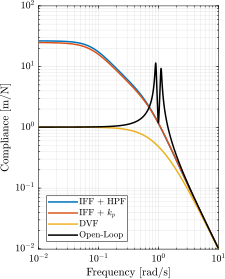
\includegraphics[width=\linewidth]{figs/comp_compliance.pdf}
\caption{\label{fig:comp_compliance} Compliance}
\end{subfigure}
\hfill
\begin{subfigure}[c]{0.49\linewidth}
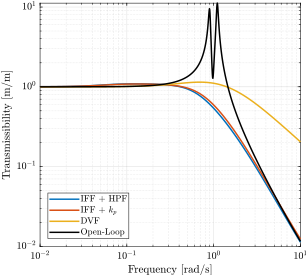
\includegraphics[width=\linewidth]{figs/comp_transmissibility.pdf}
\caption{\label{fig:comp_transmissibility} Transmissibility}
\end{subfigure}
\hfill
\caption{Comparison of the two proposed Active Damping Techniques, \(\Omega = 0.1 \omega_0\)}
\centering
\end{figure}
\end{frame}

\begin{frame}[label={sec:org46c3efd}]{}
\vspace{8em}
\begin{center}
\Huge Thank you!
\end{center}
\vspace{8em}

Contact: \href{mailto:dehaeze.thomas@gmail.com}{dehaeze.thomas@gmail.com}
\vspace{1em}
\small \url{https://tdehaeze.github.io/dehaeze20\_contr\_stewa\_platf/}
\end{frame}
\end{document}
